% ---------------------------------------------------------------------------- %
\chapter{Test Bench}
\label{chap:testBench}
% ---------------------------------------------------------------------------- %

This  chapter presents a  brief overview  of the  test bench and  provides a
step-by-step  guide on how to  put it  into operation. 

A detailled list  of all the devices, components and  software which were used
to obtain  the measurements  from Chapter  \ref{chap:results} is  given, along
with information on how to make all those pieces work.  This chapter therefore
answers  the  questions  \emph{What did  we  use,  and  how  does it  all  fit
together?}, whereas  the measurement  methodology (\emph{What  did we  do with
it?}) will be answered in the next chapter.

Fundamentally,   there   are   two    kinds   of   measurements: Digital   and
analog. The  digital  measurements consist  of  the  bit stream,  whereas  the
analog  measurements   are  concerned   with  measuring   the  pre-amplifier's
characteristics. For the most  part, the test benches for  these two scenarios
are identical.  The  primary difference is that for  the digital measurements,
the bit  stream is  measured on  the GPIO pins  of the  \raspi, while  for the
analog measurements, data  is obtained from oscilloscope. This can  be done in
multiple  ways; the  test bench  as implemented  in this  project is  based on
remote-controlling the oscilloscope from a computer.

Unless otherwise  noted, the information  presented in the  following sections
applies to both types of measurements.

% ---------------------------------------------------------------------------- %
\section{Hardware and Component List}
\label{sec:hwList}
% ---------------------------------------------------------------------------- %

\begin{centering}
\begin{xtabular}{
    >{\small}p{50mm}
    >{\small}p{8mm}
    >{\small}p{65mm}
}
    \toprule
    \textsc{Item}    &
    \textsc{Count}   &
    \textsc{Notes}   \\
    \midrule

    HP 33120A Arbitrary Waveform Generator  &
    2                                       &
    For generating input signal and clock   \\
 
    Keysight 34465A Tabletop Multimeter                     &
    3                                                       &
    Monitoring \signal{VGNDA}, \signal{VIN}, \signal{IBIAS} \\

    Aim TTi MX100TP DC Power Supply                                         &
    1                                                                       &
    Supply for \signal{VDDD}, \signal{VDDA}, \signal{VGNDA}, \signal{IBIAS} \\

    
    LeCroy waveRunner 6100A 1 GHz Oscilloscope                        &
    1                                                                 &
    Monitoring \signal{CLK}, \signal{TEST\_OUT}, \signal{SIGNAL\_OUT} \\

    Probes for LeCroy waveRunner 6100A                               &
    1                                                                &
    Measuring \signal{CLK}, \signal{TEST\_OUT}, \signal{SIGNAL\_OUT} \\

    Ethernet cable                          &
    1                                       &
    Connecting the oscilloscope to a laptop \\

    Raspberry Pi                                           &
    1                                                      &
    reading and storing bit stream (\signal{SIGNAL\_OUT}), 
    Operating System: Raspbian                             \\

    Laboratory cables with industrial plugs         &
    12                                              &
    Various connections (see diagrams and pictures) \\

    Coaxial Cables (\SI{50}{\ohm})               &
    2                                            &
    Connecting waveform generators to test board \\

    Y-adapter for coaxial cable &
    1                           &
    \\

    Breakout adapters for coaxial cables &
    3                                    &
    \\

    Measuring terminals, small &
    6                          &
    \\

    Test board &
    1          &
    \\

    Sensor IC                       &
    10                              &
    Chips used: C1V1 through C1V10  \\

    USB $\rightarrow$ RS232 adapters                  &
    2                                                 &
    For controlling the waveform generators from a PC \\

    USB cables                                        &
    2                                                 &
    For controlling the waveform generators from a PC,
    USB A $\rightarrow$ USB-B                         \\

    Computer                                                  &
    1                                                         &
    Remote-control for oscilloscope and waveform generators,
    Operating System: Linux  or *BSD with  a bash-compatible
    shell and the necessary Python libraries                  \\

    Hand-held multimeter                         &
    1                                            &
    For monitoring various parameters as needed. \\

    \bottomrule
\end{xtabular}
\end{centering}
\todo[inline]{%
        Which devices and components have been used, and for which purposes?%
}

% ---------------------------------------------------------------------------- %
\section{Assembly}
\label{sec:assembly}
% ---------------------------------------------------------------------------- %

This  section  describes  how  the  hardware listed  above  is  connected  and
configured. A   schematic   of  the   complete   test   bench  is   shown   in
\fref{fig:experimentDiagram}.

\begin{figure}
    \sisetup{range-phrase = { \ldots }}
\sisetup{list-pair-separator = {/}}

\begin{circuitikz}[x=1mm,y=1mm]

    % ------------------------------------------------------------------------ %
    % Test Board
    % ------------------------------------------------------------------------ %
    \draw (0,0) -- (50,0) -- (50,29) -- (0,29) -- cycle;

    % Left-hand side Plugs
    \foreach \y in {0,...,6} {%
        \draw (0,\y*3.5+2.5) -- (8,\y*3.5+2.5) -- (8,\y*3.5+5.5) -- (0,\y*3.5+5.5) -- cycle;
    };

    % CLK plug
    \draw (23,27.5) -- (27,27.5) -- (27,28.5) -- (23,28.5) -- cycle;
    \foreach \x in {0,...,3} {%
        \fill (23.25+\x,27.75) -- (23.25+\x+0.5,27.75) -- (23.25+\x+0.5,28.25) -- (23.25+\x,28.25) -- cycle;
    }

    % Signal out Plug
    \draw (29,27.5) -- (33,27.5) -- (33,28.5) -- (29,28.5) -- cycle;
    \foreach \x in {0,...,3} {%
        \fill (29.25+\x,27.75) -- (29.25+\x+0.5,27.75) -- (29.25+\x+0.5,28.25) -- (29.25+\x,28.25) -- cycle;
    }

    % DIP switch housing
    \draw (22,24) -- (32,24) -- (32,26) -- (22,26) -- cycle;
    \foreach \x in {1,...,9} {%
        \draw (\x+22,24) -- (\x+22,26);
    }

    % DIP Switches
    \foreach \x in {0,...,9} {%
        \fill (22+\x+0.25,24.5) -- (22+\x+0.75, 24.5) -- (22+\x+0.75,25) -- (22+\x+0.25,25) -- cycle;
    }


    % ------------------------------------------------------------------------ %
    % RasPi
    % ------------------------------------------------------------------------ %
    \draw (10,50) -- (50,50) -- (50,70) -- (10,70) -- cycle;

    % GPIO
    \foreach \x in {0,...,39} {%
        \fill (49.5-\x*0.6667-0.25,50.25) -- (49.5-\x*0.66675-0.25-0.35,50.25) -- (49.5-\x*0.66675-0.25-0.35,50.5) -- (49.5-\x*0.6667-0.25,50.5);
        \fill (49.5-\x*0.6667-0.25,50.875) -- (49.5-\x*0.66675-0.25-0.35,50.875) -- (49.5-\x*0.66675-0.25-0.35,51.125)   -- (49.5-\x*0.6667-0.25,51.125);
    }

    % ------------------------------------------------------------------------ %
    % Voltage and Current Sources
    % ------------------------------------------------------------------------ %

    % Supply Voltages
    \draw (0,25) -- (-5,25) node[circ] {}-- (-20,25) to[american voltage source,l_=\scriptsize{\SI{3}{\volt}},-*] (-20,40);

    \draw (-5,25) -- (-5,21.5) -- (0,21.5);
    \draw (0,18) -- (-40,18) to[american voltage source,l_=\scriptsize{\SI{1.5}{\volt}},-*] (-40,40);

    \draw (-60,40) to[american current source,l^=\scriptsize{\SI{120}{\micro\ampere}},*-] (-60,11) -- (0,11);

    % GND Line
    \draw (0,4) -- (-70,4) -- (-70,40) -- (25.125,40) -- (25.125,50.25);

    % CLK
    \draw (0,40) node[circ]{} -- (0,35) to[square voltage source,-*] (23.5,35) -- (23.5,28);
    \draw (23.5,35) -- (28.375,35) -- (28.375,50.25);

    % ------------------------------------------------------------------------ %
    % Signal out line
    % ------------------------------------------------------------------------ %
    \draw (30.5,28) -- (30.5,50.25);


    \draw (-70,4) node[ground]{} node[circ]{};

    %\foreach \ini [evaluate=\ini as \inieval using 2*\ini] in {0,...,6}
    %\draw[ultra thick,cyan] (\inieval,0) -- ++(0,1) -| (\inieval+1,0) -- (\inieval+2,0);
\end{circuitikz}


    \caption{%
        Experimental setup  with connections.  \emph{Note}: Drawing not
        finalized yet.%
    }
    \label{fig:experimentDiagram}
\end{figure}

\todo[inline]{How was the hardware set up? What was connected to what?}
\todo[inline]{Hardware configuration (buttons, switches, ...}
\todo[inline]{Software configuration (Raspi, python, bash, ...)}

% ---------------------------------------------------------------------------- %
\subsection{Sensor Test Board}
\label{subsec:testBoard}
% ---------------------------------------------------------------------------- %

The test board provides a platform for easy operation and configuration of the
sensor chip. It has  inputs for the various supply voltages,  a socket for the
chip itself  and outputs various signals. The  full list of the  chip's pinout
can be found in table \ref{tab:topLevelPins}.

\todo[inline]{DIP Switches}
\todo[inline]{Socket operation}
\todo[inline]{plug connections}
\todo[inline]{safety precautions}
\todo[inline]{schematic in appendix}

\begin{figure}
    \centering
    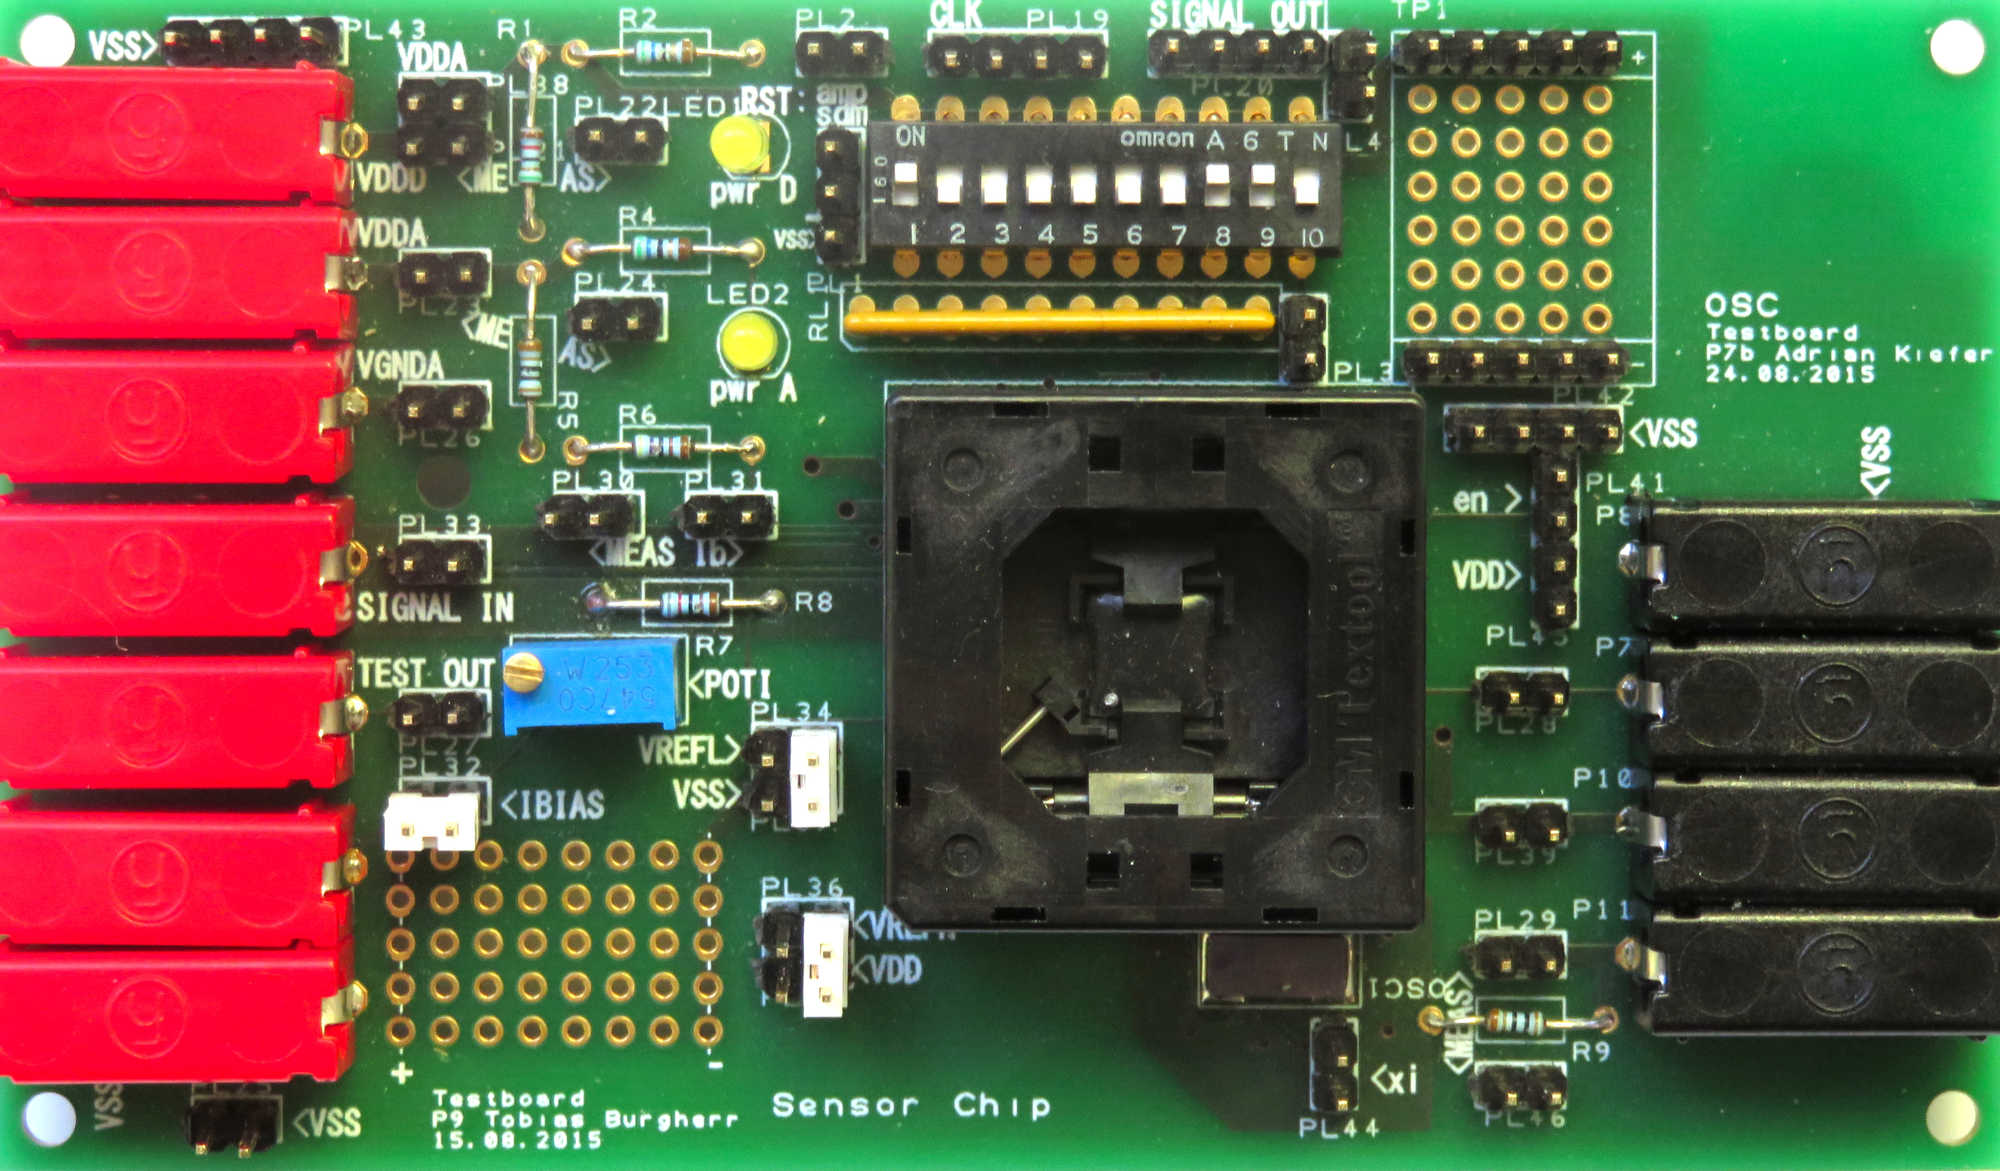
\includegraphics[width=0.9\textwidth]{images/pcb/pcbOverview}
    \caption{The test board.}
    \label{fig:testBoard}
\end{figure}

\begin{table}
    \centering
    \caption{Sensor chip toplevel pins}
    \label{tab:topLevelPins}
    \scriptsize
    \sisetup{list-pair-separator = { or }}
    \rowcolors{2}{solarized-base3}{white}
    \begin{tabular}{>{\fontfamily{jkptt}\selectfont}l>{\fontfamily{jkptt}\selectfont}lp{30mm}lp{30mm}} \\
    %\begin{tabular}{>{\fontfamily{lmtt}\selectfont}l>{\fontfamily{lmtt}\selectfont}lp{30mm}lp{30mm}} \\
        \toprule
        \textnormal{\textsc{Pin \#}} & \textnormal{\textsc{Name}}                  & \textsc{Description} & \textsc{Value} & \textsc{Note} \\
        \midrule
        39 & vin                     & analog input signal                         & \SIrange{0.5}{2.5}{\volt} & \\
        25 & bit\_stream             & digital output signal                       & \SIlist{0;3}{\volt}       & \\
        34 & clk                     & clock                                       & \SIlist{0;3}{\volt}       & \\
        36 & sdm\_rst                & pulse to reset the $\Sigma\Delta M$         & \SIlist{0;3}{\volt}       & short pulse is enough (min $T_C$) \\
        41 & vgnda                   & analog ground                               & \SI{1.5}{\volt}           & \\
        48 & vrefh                   & high reference voltage                      & \SI{3}{\volt}             & \\
        47 & vrefl                   & low reference voltage                       & \SI{0}{\volt}             & \\
        46 & ibias                   & bias current                                & \SI{120}{\micro\ampere}   & $24 \cdot 5 \cdot 1$, internally reduced by 120 \\
        43 & sc\_amp\_vout\_test\_en & enables test output after preamp            & \SIlist{0;3}{\volt}       & \SI{0}{\volt}: off, \SI{3}{\volt}: on\\
        44 & sc\_amp\_vout\_test     & test output after preamp                    & \SIrange{0.5}{2.5}{\volt} \\
        33 & sc\_amp\_rst\_ext\_en   & enables external reset input for the preamp & \SIlist{0;3}{\volt}       & \SI{0}{\volt}: off, \SI{3}{\volt}: on\\
        32 & sc\_amp\_rst\_ext       & external reset input for the preamp         & \SIlist{0;3}{\volt}       & Internally synced to \signal{clk}. Needs \signal{en} signal. \\
        35 & sc\_amp\_pos\_neg\_amp  & positive or negative gain                   & \SIlist{0;3}{\volt}       & \SI{0}{\volt}: positive, \SI{3}{\volt}: negative \\
        28 - 31 & sc\_amp\_csel<3:0> & set gain                                    & \SIlist{0;3}{\volt}       & See table TODO \\
        27 & sc\_amp\_en             & enable preamp                               & \SIlist{0;3}{\volt}       & \SI{0}{\volt}: off, \SI{3}{\volt}: on\\
        26 & sah\_sdm\_en            & enable $\Sigma\Delta M$ S/H bock            & \SIlist{0;3}{\volt}       & \SI{0}{\volt}: off, \SI{3}{\volt}: on\\
        42 & vdda                    & analog positive power supply                & \SI{3}{\volt}             & \\
        37 & vddd                    & digital positive power supply               & \SI{3}{\volt}             & \\
        40 & vss                     & analog and digital negative power supply    & \SI{0}{\volt}             & \\
        \bottomrule
    \end{tabular}
    \sisetup{list-pair-separator = { and }}
\end{table}

% ---------------------------------------------------------------------------- %
\subsection{DC Power Supply}
\label{subsec:dcPower}
% ---------------------------------------------------------------------------- %
\todo[inline]{reference to user manual}
\todo[inline]{Connections}
\todo[inline]{control output voltages with voltmeter}

The  \dcsupp~ has  three  independent direct  voltage  outputs. They are  used
to  supply \signal{VDDD},  \signal{VDDA},  \signal{VREFH}, \signal{VGNDA}  and
\signal{IBIAS}\footnotemark. Since the output current can only be limited, but
not  directly  set, the  bias  current  output  is  fed directly  through  one
of  the Keysight  tabletop  multimeters. The bias  current  is then  monitored
and  the  \dcsupp's  output  voltage  (and/or the  variable  resistor  on  the
test  board)  adjusted as  needed  to  achieve  the  desired bias  current  of
\SI{120}{\uA} as per Table \ref{tab:topLevelPins}.

\footnotetext{%
    All  \SI{3}{V} signals  are  fed  from the  same  output  and bridge  with
    jumpers  on the  test board. This  concerns \signal{VDDD},  \signal{VDDA},
    \signal{VREFH} and \signal{VGNDA}.
}

% ---------------------------------------------------------------------------- %
\subsection{Waveform Generators}
\label{subsec:33120A}
% ---------------------------------------------------------------------------- %
\todo[inline]{reference to user manual}
\todo[inline]{scripts, connections}
\todo[inline]{control output voltages with voltmeter}

The  \funcgen  s  are  controlled  remotely via  their  RS232  interface  from
a  computer  (through  RS232  $\rightarrow$   USB-A  adapters)  and  a  Python
script   (\code{33120A.py},  see   Appendix  \ref{app:chap:scripts}   on  page
\pageref{app:chap:scripts}).

Before usage, the  script needs to be configured. The  two waveform generators
will  show up  in the  computer's  device tree  and their  identities must  be
entered into the script in the \code{SETTINGS} section:

\begin{minted}{python}
# ------------------------------------------------------------------------ #
# SETTINGS                                                                 #
# ------------------------------------------------------------------------ #
CLK_DEVICE = '/dev/ttyUSB1'
DC_DEVICE  = '/dev/ttyUSB0'
\end{minted}

Whichever  device   registered  with  the   PC  first  will  have   the  lower
\code{ttyUSB<N>} number. If other  devices are connected to  the computer, the
numbers will of course be higher than \code{0} and \code{1}, respectively.

After successful configuration, the waveform generators can be controlled from
the command line like so\footnotemark:

\begin{minted}{shell}
$ ./33120A.py --clock=32e3
$ ./33120A.py --voltage=1.8
\end{minted}

The script will then select either the \signal{CLK} \signal{SIGNAL\_IN} device
and adjust  its output as specified. In  this case, the sampling  rate for the
test board  is set  to \SI{32}{\kilo\hertz}  and the DC  voltage on  the other
generator  is set  to \SI{1.8}{\volt}. More  information can  be found  in the
script itself.

The \signal{CLK} device  will always output a square wave  with voltage levels
\SI{0}{volt} and \SI{3}{\volt}, as per table \ref{tab:topLevelPins}.

If needed,  the script can  easily be extended  to output any  other arbitrary
signal. The full  list of available commands  can be obtained from  the 33120A
operator's manual.
\todo[inline]{source}

\footnotetext{%
    This requires  the executable bit  to be set  on the file:  \code{chmod +x
    33120A.py}.%
}


% ---------------------------------------------------------------------------- %
\subsection{Multimeters}
\label{subsec:34465A}
% ---------------------------------------------------------------------------- %

Three \emph{Keysight 34465A} multimeters are used. One for monitoring the bias
current, a second for monitoring the voltage for the input signal, and a third
one for monitoring the reference voltage (analog ground).

The wiring connections are depicted in figure \ref{fig:multimeterConnections}.

\begin{figure}
    \centering
    \missingfigure{multimeters}
    \caption{Multimeter connections}
    \label{fig:multimeterConnections}
\end{figure}

No  further  special  configuration  is  needed  on  the  multimeters  besides
setting  them  to   the  correct  measurement  modes   (voltage  and  current,
respectively). Care must be  taken though when setting the range  for the bias
current measurement. \SI{120}{\micro\ampere} is right  on the edge between two
measurement ranges (\si{\micro\ampere}  and \si{\milli\ampere}, respectively),
and the measurement results between these two ranges are not identical. In our
measurements, the device is set to the millivolt range.

\todo[inline]{reference to user manual}


% ---------------------------------------------------------------------------- %
\subsection{Oscilloscope}
\label{subsec:oscilloscope}
% ---------------------------------------------------------------------------- %

\todo[inline]{connections}
\todo[inline]{configuration}
\todo[inline]{script}
\todo[inline]{quirks}


The oscilloscope  is used for  monitoring the clock,  the bit stream,  and for
acquiring measurment data for the preamp via the test output pin.

% ---------------------------------------------------------------------------- %
\subsubsection{Clock and Bit Stream}
\label{subsubsec:clockBitstream}
% ---------------------------------------------------------------------------- %

Measuring clock  and bit  stream is straightforward: The  oscilloscopes probes
are  connected  to the  corresponding  pins  on  the  test board  as  depicted
in figures  \ref{fig:clockBitStreamProbes} and \ref{fig:clockBitStreamScreen},
respectively.

\begin{figure}
    \centering
    \missingfigure{probe connections}
    \caption{Clock and bit stream measurement}
    \label{fig:clockBitStreamProbes}
\end{figure}

\begin{figure}
    \centering
    \missingfigure{Clock and bit stream, screenshot}
    \caption{Clock and bit stream measurement, screenshot}
    \label{fig:clockBitStreamScreen}
\end{figure}

If  the   clock  and   bit  stream   do  not  look   as  depicted   in  figure
\ref{fig:clockBitStreamScreen}, common  errors are a  disabled sample-and-hold
circuit,  an  incorrect clock  voltage  (particularly  its  DC offset)  or  an
incorrect bias current.


% ---------------------------------------------------------------------------- %
\subsubsection{Analog Measurements of Preamp}
\label{subsubsec:analogMeasurements}
% ---------------------------------------------------------------------------- %

Performing  analog measurements  of  the pre-amplifier  is  a noticeably  more
involved process. A measurement  probe is connected to the test  output pin on
the test board as shown in figure \ref{fig:probePreamp}.

\begin{figure}
    \centering
    \missingfigure{Probe connection preamp measurement}
    \caption{Probe connection preamp measurement}
    \label{fig:probePreamp}
\end{figure}

Besides the  oscilloscope itself,  a laptop  is used  to remotely  control the
oscilloscope and  the two function generators  (one for the clock  and for the
input signal, respectively).

The  connection  between  the  Oscilloscope  and  the  laptop  is  established
via  ethernet, with  each  device being  assigned a  fixed  IP. The laptop  is
configured  to match  the  oscilloscope's network  settings. How to  configure
the  laptop  is  outline  in Section  \ref{subsec:laptop},  starting  on  page
\pageref{subsec:laptop}.


After  having  successfully  established   a  connection  between  laptop  and
oscilloscope, a  collection of  three scripts  is used  to configure  the test
setup and acquire the measurement data:

\begin{itemize}\tightlist
    \item 
        A shell wrapper script, 
    \item
        \code{33120A.py}: For controlling the waveform generators (see section
        \ref{subsec:33120A})
    \item 
        \code{initWaveRunner.py}: resets and initializes the oscilloscope with
        a given configuration.
    \item 
        \code{configWaveRunner.py}:   configures  various   settings  on   the
        oscilloscope.
    \item 
        \code{acquireWaveRunnerData.py}:   performs   measurements   via   the
        oscilloscope.
\end{itemize}


The  python  scripts   are  mostly  self-explanatory  with   aid  of  LeCroy's
documentation   found  in   \cite{ref:WR:opMan},  \cite{ref:WR:gettingStarted}
and    \cite{ref:WR:remoteControl}. A   detailled    explanation   of    their
implementation   will   therefore   be   ommitted,   and   instead   a   brief
outline   of   each   script's   purpose  and   usage   is   provided.    They
can    be    found    in    Appendices    \ref{sec:app:waveRunner:initialize},
\ref{sec:app:waveRunner:config} and \ref{sec:app:waveRunner:acquire}, starting
on page \pageref{sec:app:waveRunner:initialize}.

The initialization script  resets the oscilloscope and  configures the trigger
channel, trigger level, trigger flank,  time division, which traces to display
and sets the DC coupling of the channels to a resistance of \SI{1}{\mega\ohm}.

\code{configWaveRunner.py} is used  to set the horizontal  (time) and vertical
(voltage) divisions on the oscilloscope,  as well as the vertical offset. This
is necessary because the oscilloscope will only store measurement data for the
section of any given trace which is being shown on the display. Any meaurement
points which  are not on  the oscilloscope's display will  not be stored  in a
measurement file. Although this is a  bit cumbersome and counter-intuitive, it
does have  the advantage that  one can see  immediately if something  has been
incorrectly configured during  the measurement process, as  the display output
will then be incorrect.

\code{acquireWaveRunnerData.py}  executes   the  actual  measurement   on  the
oscilloscope  for a  given channel. The  measurement results  are stored  in a
text-file, which is then downloaded to the laptop.

The entire process is controlled via  a shell wrapper script. This script will
be explained  in more  detail in the  following paragraphs. There  are various
versions of  the script for  different measurements,  but they all  follow the
same outline.

For each measurement run, the chip  number, the gain (sign and absolute value)
and the channel which  is connected to the test output on  the test board must
be set.  Furthermore, the target directory  in which the measurement data will
be stored  on the PC is  set according to  the chip number and  gain settings.
There  is  also  an  optional  flag  for  resetting  the  oscilloscope  before
performing the measurements,  if so desired. In the following  example, a gain
of \code{+1} will be measured for chip number 1:

\begin{minted}{shell}
CHIP='chip01'
SIGN='+'
CHANNEL='3'
GAIN='1'
DATA_DIR="data/${CHIP}Gain${SIGN}$(printf '%02d' $GAIN)"
RESET='0' # 1: reset and initialize the oscilloscope
\end{minted}

Before actually performing any measurements,  the script will display a series
of  messages to  the user,  accounting  for a  few quirks  of the  setup. This
minimizes user error and ensures that time is not wasted on measurements being
useless due to erroneous configurations.

The first message concerns the number  of sample points which the oscilloscope
is set to acquire. This  must be set to \num{500} kilo  samples per second, as
shown in  Figure \ref{fig:kilosamples}. If this  is not done,  the measurement
data will show aliasing, resulting in useless data.

\begin{figure}
    \centering
    \missingfigure{kilosamples}
    \caption{Set sample rate on oscilloscope}
    \label{fig:kilosamples}
\end{figure}

The  next  two  messages  concern  the  measurement  files  which  are  stored
on   the  oscilloscope.    They   follow   a  naming   scheme   of  the   form
\code{C<ChannelNo>Trace<FileNo>.txt},   starting   at  file   zero   (example:
\code{C2Trace00002.txt}  for the  third  file for  channel 2). Each  channel's
counter is independent of the  other channels' counters. The counter for these
file names  will keep incrementing,  regardless of any remote  commands, until
they are manually reset via the Oscilloscope's graphical user interface.

To avoid needing to manually reset  this counter between each measurement, the
script maintains  its own  counter to  match the  oscilloscope's. Between each
measurement  run (i.e.  each script  execution), manual  intervention via  the
oscilloscope's GUI is necessary to reset the oscrilloscope's counter, as shown
in figure \ref{fig:fileCounterReset}.

\begin{figure}
    \centering
    \missingfigure{Counter Reset}
    \caption{Resetting the file counter on the oscilloscope}
    \label{fig:fileCounterReset}
\end{figure}

The  next   step  in   the  script's  execution   is  performing   the  actual
measurements. Various  settings  are  hard-coded  into  the  script  for  this
purpose. Firstly,  the   appropriate  time   divisions  for   configuring  the
oscilloscope's display\footnotemark:

\begin{minted}{shell}
declare -A timeDivs
timeDivs[32e3]='5'
timeDivs[96e3]='2.5'
timeDivs[256e3]='1'
\end{minted}

\footnotetext{
    These  values were  obtained by  trial and  error to  generate a  sensible
    display output.
}

Additionally, the list of amplitudes to be used for the input voltages:

\begin{minted}{shell}
declare -a ampls=(0.5 0.7 0.9 1.1 1.3 1.5 1.7 1.9 2.1 2.3 2.5)
\end{minted}

Each input voltage (including the gain's  sign) is assigned a voltage division
and a time division for the oscilloscope's display settings\footnotemark:

\begin{minted}{shell}
declare -A voltDivs
voltDivs[+0.5]='200'
voltDivs[+0.7]='200'
voltDivs[+0.9]='100'
...
voltDivs[-2.1]='100'
voltDivs[-2.3]='200'
voltDivs[-2.5]='200'

declare -A offsets
offsets[+0.5]='-1000'
offsets[+0.7]='-1100'
offsets[+0.9]='-1200'
...
offsets[-2.1]='-1200'
offsets[-2.3]='-1100'
offsets[-2.5]='-1000'
\end{minted}

\footnotetext{
    Also determined by trial and error.
}

Now, everything is  ready to perform the measurements, tying  together all the
scripts and configurations which have been mentioned so far:

\begin{minted}{shell}
i=0
mkdir -p "$DATA_DIR"
for clk in 32e3 96e3 256e3;do
    ./33120A.py --clock=$clk
    sleep 0.25 # give the function generator time to settle
    ./configWaveRunner.py --tdiv=${timeDivs[$clk]}

    # Run through DC ramp
    for ampl in "${ampls[@]}";do
        ./33120A.py --voltage="$ampl"
        sleep 0.25
        ./configWaveRunner.py \
            --vdiv=${voltDivs[${SIGN}${ampl}]} \
            --offset=${offsets[${SIGN}${ampl}]}
        sleep 2 # Give the oscilloscope time to do configure
        printf 'Acquiring trace for %s Hz and %s V\n' $clk $ampl
        ./acquireWaveRunnerData.py \
            --channel="C${CHANNEL}" \
            --remotefile="C${CHANNEL}Trace$(printf '%05d' $i).txt" \
            --localfile="${DATA_DIR}/${CHIP}-gain${SIGN} \
                $(printf '%02d' ${GAIN})-${fsStrings[$clk]}-${ampl}V.txt"
        i=$((i+1))
    done
done
\end{minted}

For each  measurement series, one  target directory  is created, in  which one
file for each clock frequency and  input voltage is generated. These files can
then be processed as outlined in Chapter \ref{chap:results}.


% ---------------------------------------------------------------------------- %
\subsection{Raspberry Pi}
\label{subsec:raspi}
% ---------------------------------------------------------------------------- %

\todo[inline]{software installation}
\todo[inline]{measurement programs}
\todo[inline]{pin connections}
\todo[inline]{Network config}


% ---------------------------------------------------------------------------- %
\subsection{Laptop}
\label{subsec:laptop}
% ---------------------------------------------------------------------------- %

This section outlines the prerequisites, configuration and usage of a computer
which is  used to  control the  measurement process. A laptop  is used  in our
case, but  any computer with  a network  and at least  two USB ports  (for the
waveform generators) can be used.


% ---------------------------------------------------------------------------- %
\subsubsection{Prerequisites}
\label{subsubsec:laptop:prereqs}
% ---------------------------------------------------------------------------- %

For controlling the test bench, a laptop running Linux is used. Fundamentally,
other configurations are likely also  possible. Any Bash version 4.0 and newer
should  be able  to execute  the wrapper  scripts (associated  arrays must  be
supported). Even Windows 10  has Bash as well  these days \cite{ref:W10:bash},
though compatibility with our script suite has not been verified).

Besides  Bash  >4.0 support,  Python  3  must  be  installed, along  with  the
following modules:

\begin{itemize}\tightlist
    \item
        \code{serial}: For communicating with the waveform generators
    \item
        \code{vxi11}: For communicating with the oscilloscope
\end{itemize}

These  modules can  either be  installed via  pip or  via your  distribution's
package manager.


% ---------------------------------------------------------------------------- %
\subsubsection{Ethernet Configuration}
\label{subsubsec:laptop:netconf}
% ---------------------------------------------------------------------------- %

For  communicating  with  the  oscilloscope via  ethernet,  a  static  network
connection is used,  corresponding to the settings on  the oscilloscope (which
can be checked via the network dialog in Windows XP).

On the  machine used in our  measurements (a Macbook Pro  running Arch Linux),
this is done via \code{netctl} as follows\footnotemark:

\begin{minted}{text}
Description='WaveRunner Oscilloscope Ethernet Connection'
Interface=ens9                                                                                                                                                                                            
Connection=ethernet                                                                                                                                                                                       
IP=static                                                                                                                                                                                                 
Address=('169.254.14.1/16')                                                                                                                                                                               
\end{minted}

\footnotetext{
    Make  sure   \emph{not}  to  set   a  \code{Gateway}  parameter   in  this
    configuration,  or the  laptop will  try to  access the  internet via  the
    oscilloscope, which will obviously fail.
}

The  \code{Interface} parameter  needs to  be  adjusted to  the machine  which
is  being  used. A  list  of   available  interfaces  can  be  displayed  with
\code{ip  addr}  on  systems  which have  the  \code{iproute2}  utility  suite
\cite{ref:iproute2}  installed,  or with  \code{ifconfig}  \cite{ref:ifconfig}
on  other  *nix  operating  systems. For  further  information,  consult  your
distribution's manpages.


% ---------------------------------------------------------------------------- %
\subsubsection{SSH Configuration}
\label{subsubsec:laptop:sshconf}
% ---------------------------------------------------------------------------- %

The \raspi~  is remote-controlled via SSH  from the laptop. In order  to avoid
having to  type in  a password  for each SSH  connection attempt  (which would
become cumbersome  very quickly), SSH  key files  are used. Because this  is a
rather expansive topic  with a lot of available information,  a quick guide is
povided  here\footnotemark. These  steps are  based  on  the Arch  Linux  Wiki
\cite{ref:archWiki:SSH} , but  should work with any  reasonably modern OpenSSH
installation:

\todo[inline]{put SSH config tutorial into appendix?}

\footnotetext{
    If you already have  an SSH key pair or know how to  do this, this section
    can be  skipped, unless you wish  to generate a new  key pair specifically
    for this use.
}

First, generate a new key pair:

\begin{minted}{shell}
$ ssh-keygen
\end{minted}

The laptop is ready to properly execute our wrapper scripts as indented.
